 
Nowadays there is a growing interest on the 3D scene reconstruction field, due to the incresing computational power and the reduction of 
the costs of the capturing devices. There are a lot of differents approaches to afront the problem, there are works that perform 3D reconstruction 
from a video, from a set of images taken with an unknown camera and orientation, using active devices that project patterns of light into 
the scene, lasers, etc. 

In 3D reconstruction an important part of the problem depends of the intrinsical 
device characteristics (noise, resolution, framerate, etc), the scene or object beign captured, ilumination, the camera location and position, etc. All this factors configure different instances of the problem, difficulting the comparison and limiting the use of a common dataset, but some efforts in order to allow comparison between different algorithms has been made 
in \cite{seitz2006}, \cite{ponce2006} and \cite{scharstein2001}.

Usually the researchers estimate their systems performance comparing the generated 3D model with some 
ground truth model obtained with a high precision laser scanner. Also its common to measure the performance
 comparing some result obtained at an intermediate step of the reconstruction process with a ground truth measure, 
such as the camera estimated path with camera real path.   

%done
Reconstruction from a set of photographs without human assistance is performed in \cite{jan}, they demonstrated the first system able to deliver dense geometry for Internet scale photo collections with millions of images of an entire city within the span of a day on a single PC. They used appearance-based clustering in multiple CPU and GPU cores 
in order agrupate images corresponding to the same site, using gist features for each image along with a RGB
descriptor in order to mantain color information. They also used geo-location information available for some of 
the images. Then at each cluster they performed 3D reconstruction using only the images with mutually consistent epipolar 
geometry. From millions of images from one city they generated thousands of 3D models of buildings. See figure \ref{fig:jan}. 


\begin{figure}[h!]
\begin{center}
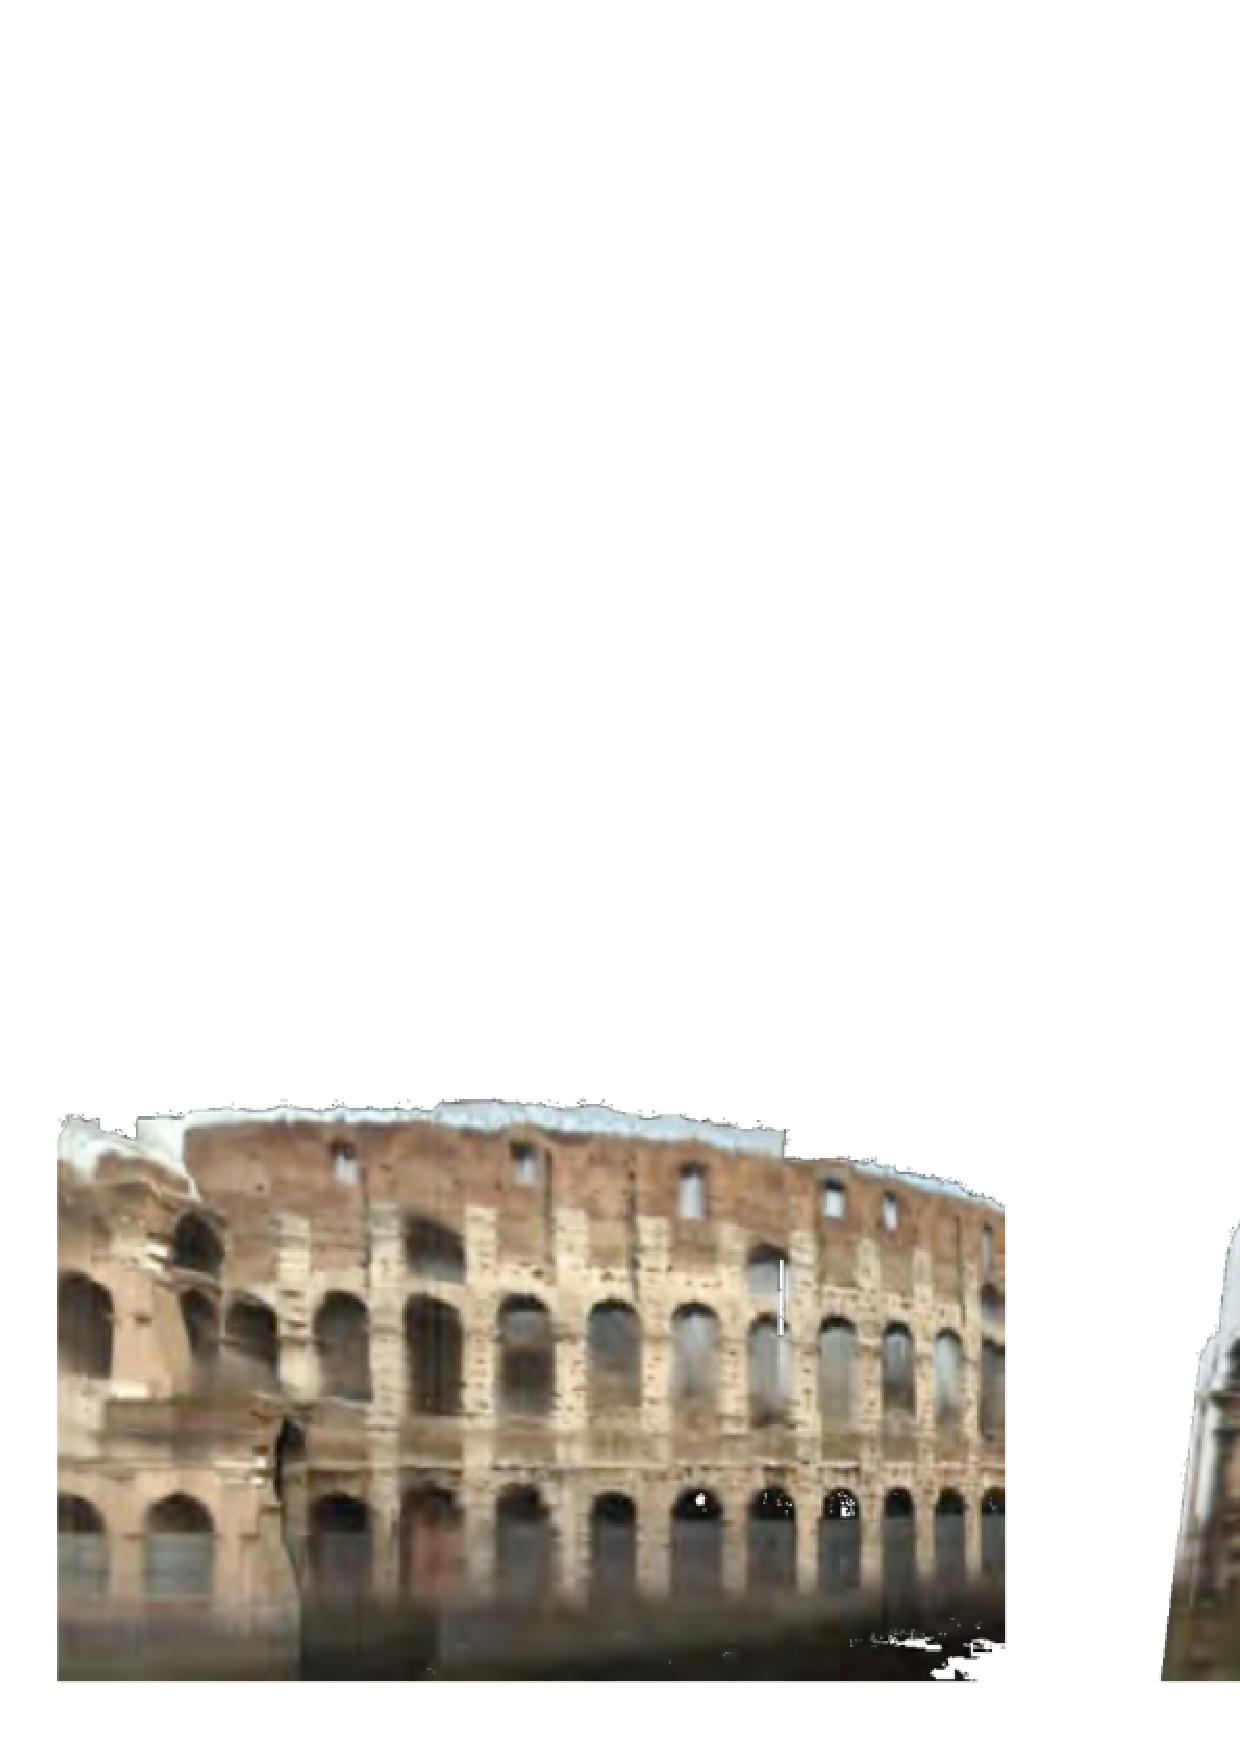
\includegraphics[scale=0.25]{images/jan}
\caption{Reconstructed 3D buildings in less than 24 hr. using 2.8 million and 2.9 million of images respectively}
\label{fig:jan}
\end{center}
\end{figure}

%done
In \cite{guangyu} an hybrid approach is used, combining a ToF (Time of Flight) camera and an grayscale camera in order to perform the reconstruction. 
The data adquisition is made rotating the object in front of the camera with a black background behind it, then they use 
SIFT (Scale Invariant Feature Transform) to find 2D feature correspondences and perform and initial alination between two consecutive frames, this alineation is 
then improved with ICP (Iterative Closest Point) algorithm. They use a 3D laser scanner in order to obtain a ground truth, obtaining a difference around of 1\% 
between their reconstructed
 models and the 3D laser models. See figure \ref{fig:guangyu}.

%put this on the correct place
Its common to find works where the method is not quantitatively evaluated 
in 3D reconstruction due to the high 
cost of a laser scanner that is used as ground truth. 


\begin{figure}[h!]
\begin{center}
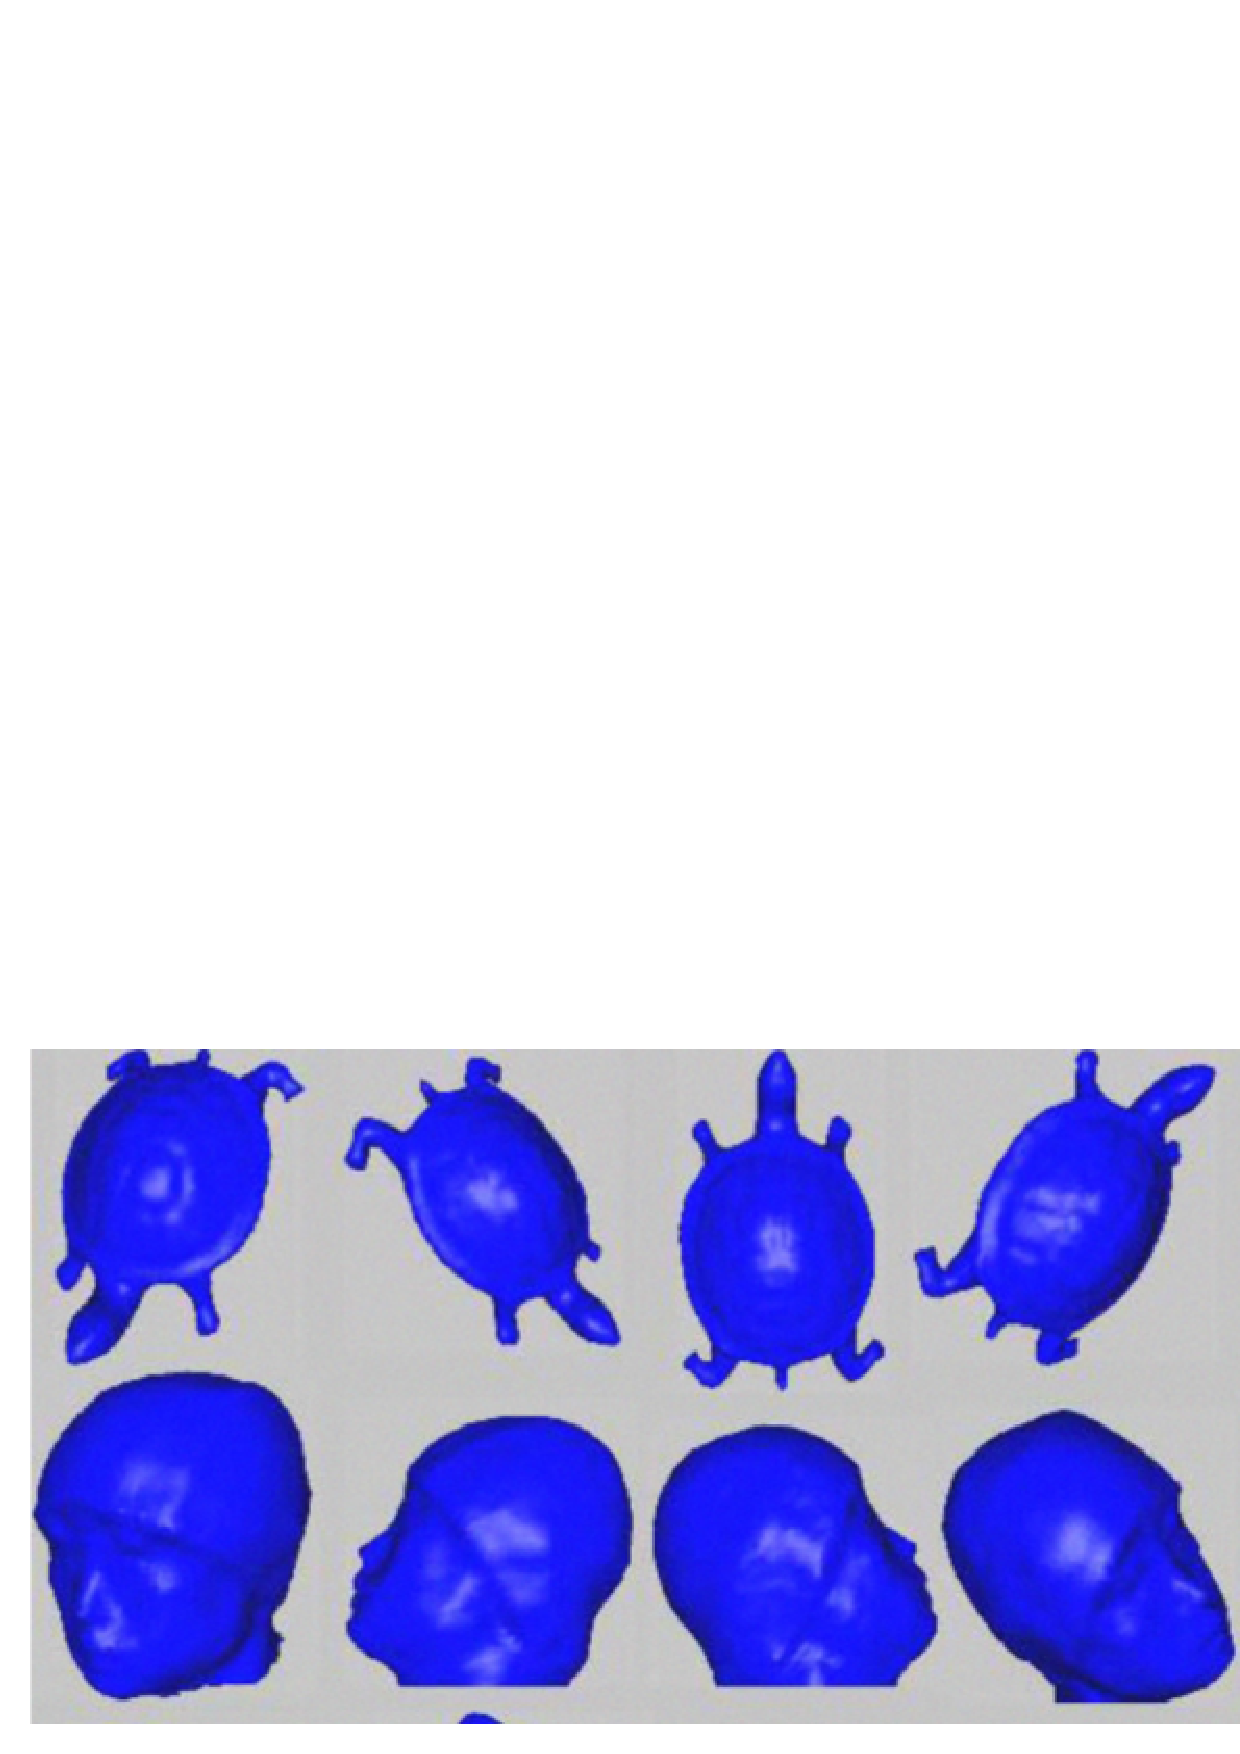
\includegraphics[scale=0.38]{images/guangyu}
\caption{3D Reconstruction of a human head and an object using ToF and RGB camera}
\label{fig:guangyu}
\end{center}
\end{figure}

%done
In \cite{may2009} a ToF camera is used in combination with an industrial robot arm (KUKA KR 16) in order to register an indor scene,
they use an improved version of the ICP algorithm called ICP Frustum, where at each iteration the points that are not overlaping with the previous frame are removed. The industrial robot arm is used to move the camera and get a ground truth camera path to evaluate the performance of their ICP algorithm. 

%Its possible to find more elaborated reconstructions using a laser scanner, but its a more expensive method. In 
%\cite{binney} there is a interesting work where a reconstruction of tree branches is performed using a laser range 
%data. They use a probabilistic approach and use knowledge about the tree structure to guide an iterative reconstruction 
%process. 

%done
In \cite{keqiang} a 3D reconstruction is performed with a laser range finder (SICK 2D ) and a mobile robot, 
using the ICP algorithm and a volumetric representation. In the matching phase of the ICP algorithm not all
 points are used, instead they just use edge points, reducing the computational cost of the process. The scene 
 representation is simplyfied removing redundant points, this is done dividing the scene into voxels and at each 
 voxel preserving just the point closer to the center. Their system produces a scene with data points evenly 
 distributed.

%revisar nuevamente
In \cite{wei} a CCD camera and a 2D laser scanner is used to perform indoor panoramic 3D reconstruction, 
they mounted both devices in a rotational stage and use a fusion algorithm to merge the depth map generated by the laser 
and the depth map generated from the CCD camera observations, the two depth maps contains noise and an intelligent merging reduce this
 noise giving more accurate information to the 3D reconstruction process. Another interesting work of indoor scene reconstruction is \cite{henry} where an RGB-D camera is used to reconstruct an indoor scene. RGB-D cameras are sensing systems that capture RGB images
 along with per pixel depth information. They use the ICP algorithm to calculate the camera location and pass to it information from 
the depth camera and  rich visual
 features along with RANSAC (RAndom SAmple Consensus) verification captured by the RGB camera. They use surfels \cite{pfister} to represent the scene. See figure \ref{fig:henry}.

\begin{figure}[h!]
\begin{center}
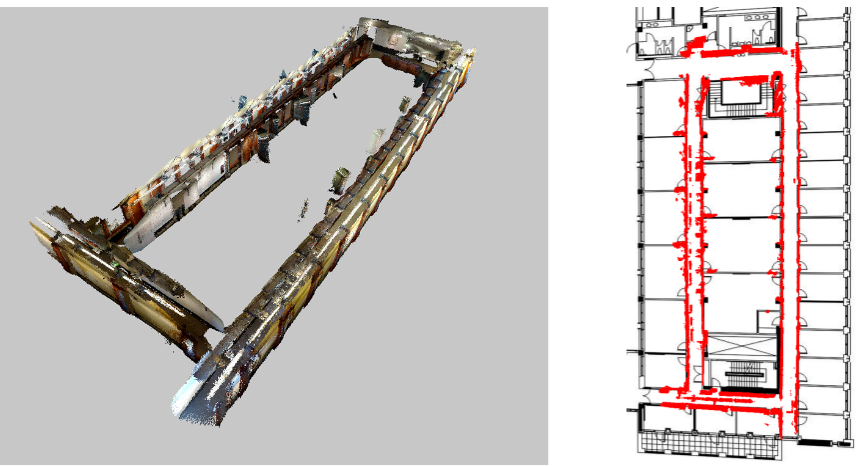
\includegraphics[scale=0.29]{images/henry}
\caption{Reconstructed 3D big indoor space}
\label{fig:henry}
\end{center}
\end{figure}

%done
In \cite{cui} a ToF camera is used to reconstruct 3D objects. A combination of 3D superresolution method with a 
probabilistic scan alignment (iterative Expectation Maximization) approach that takes into account the sensor's 
noise characteristics is used. Their method is not in real time and the resulting models contains undesirable 
artifacts due to  the noise of the captured depth maps, they use a low resolution device (176x144) and they 
improve the resolution using a superresolution method. They captured a ground truth model with a laser 3D scanner, 
obtaining differences below 1 cm in most areas between their model and the ground truth model. Their scanning 
procedure doesn't allow a freely movement around the object, the object must be at the center of view of the camera 
and the distance between the object and camera must be almost constant. A similar work can be found at \cite{schoun} where 
 a hierarchical Lukas Kanade optical flow is used for registration.
 
see figure \ref{fig:cui}.

\begin{figure}[h!]
\begin{center}
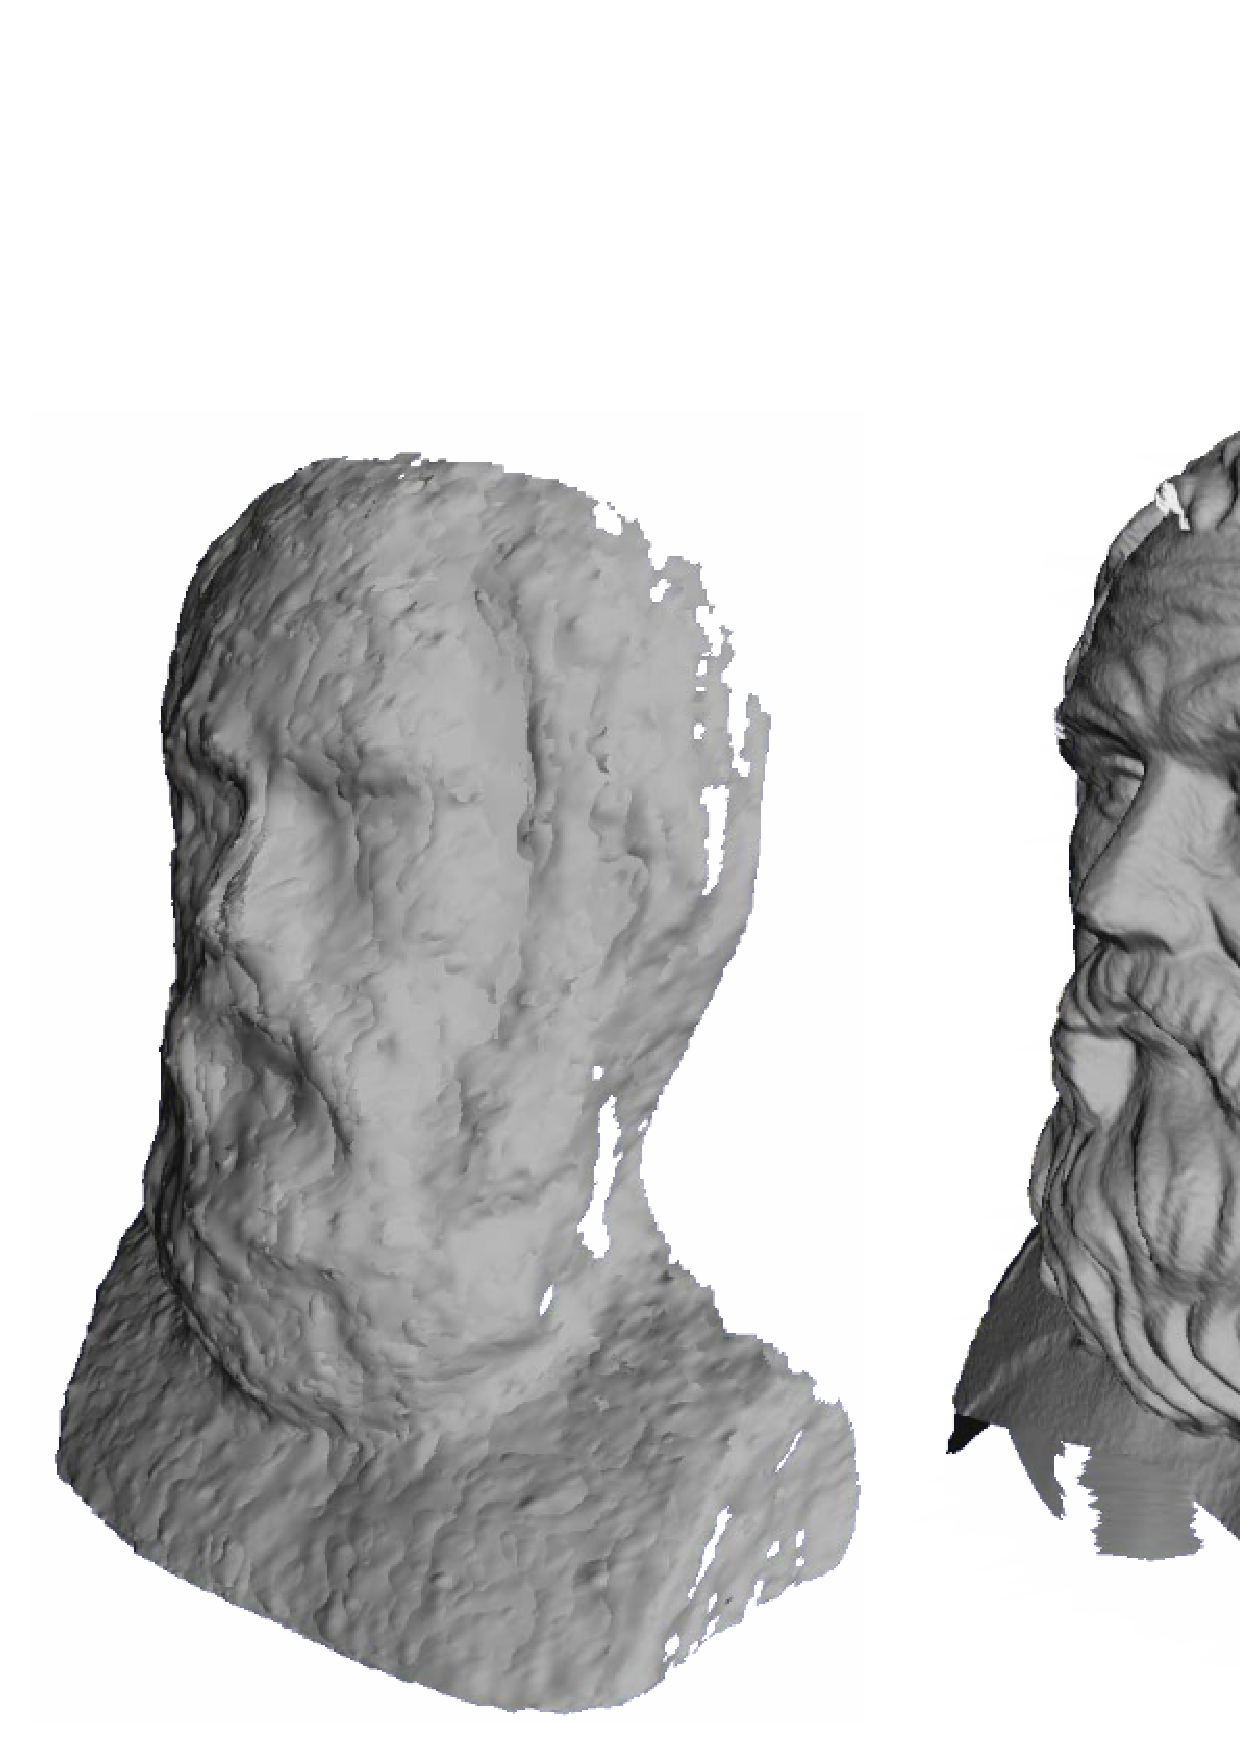
\includegraphics[scale=0.23]{images/cui}
\caption{ToF Reconstruction, Laser Reconstruction and Error Plot}
\label{fig:cui}
\end{center}
\end{figure}

 
%done
A very interesting work is made in \cite{izadi}, they use a low cost RGB-D camera (Kinect) in order to perform
the 3D reconstruction using the ICP algorithm  and a volumetric representation with a GPU in order to 
archieve real time reconstruction. The camera can move freely around the scene and the reconstruction grows in detail 
as new depth measurements are added. They apply color textures to the reconstructed scene obtaining very 
realistic models, their system is able to perform rigid body collisions 
simulations during the reconstruction, allowing thousands of virtual particles interact with the scene. Also a 
user can interact with the scene during the reconstruction process. This is one of the most advanced 
reconstruction systems, due to its uniques features.

 see figure \ref{fig:izadi}.

\begin{figure}[h!]
\begin{center}
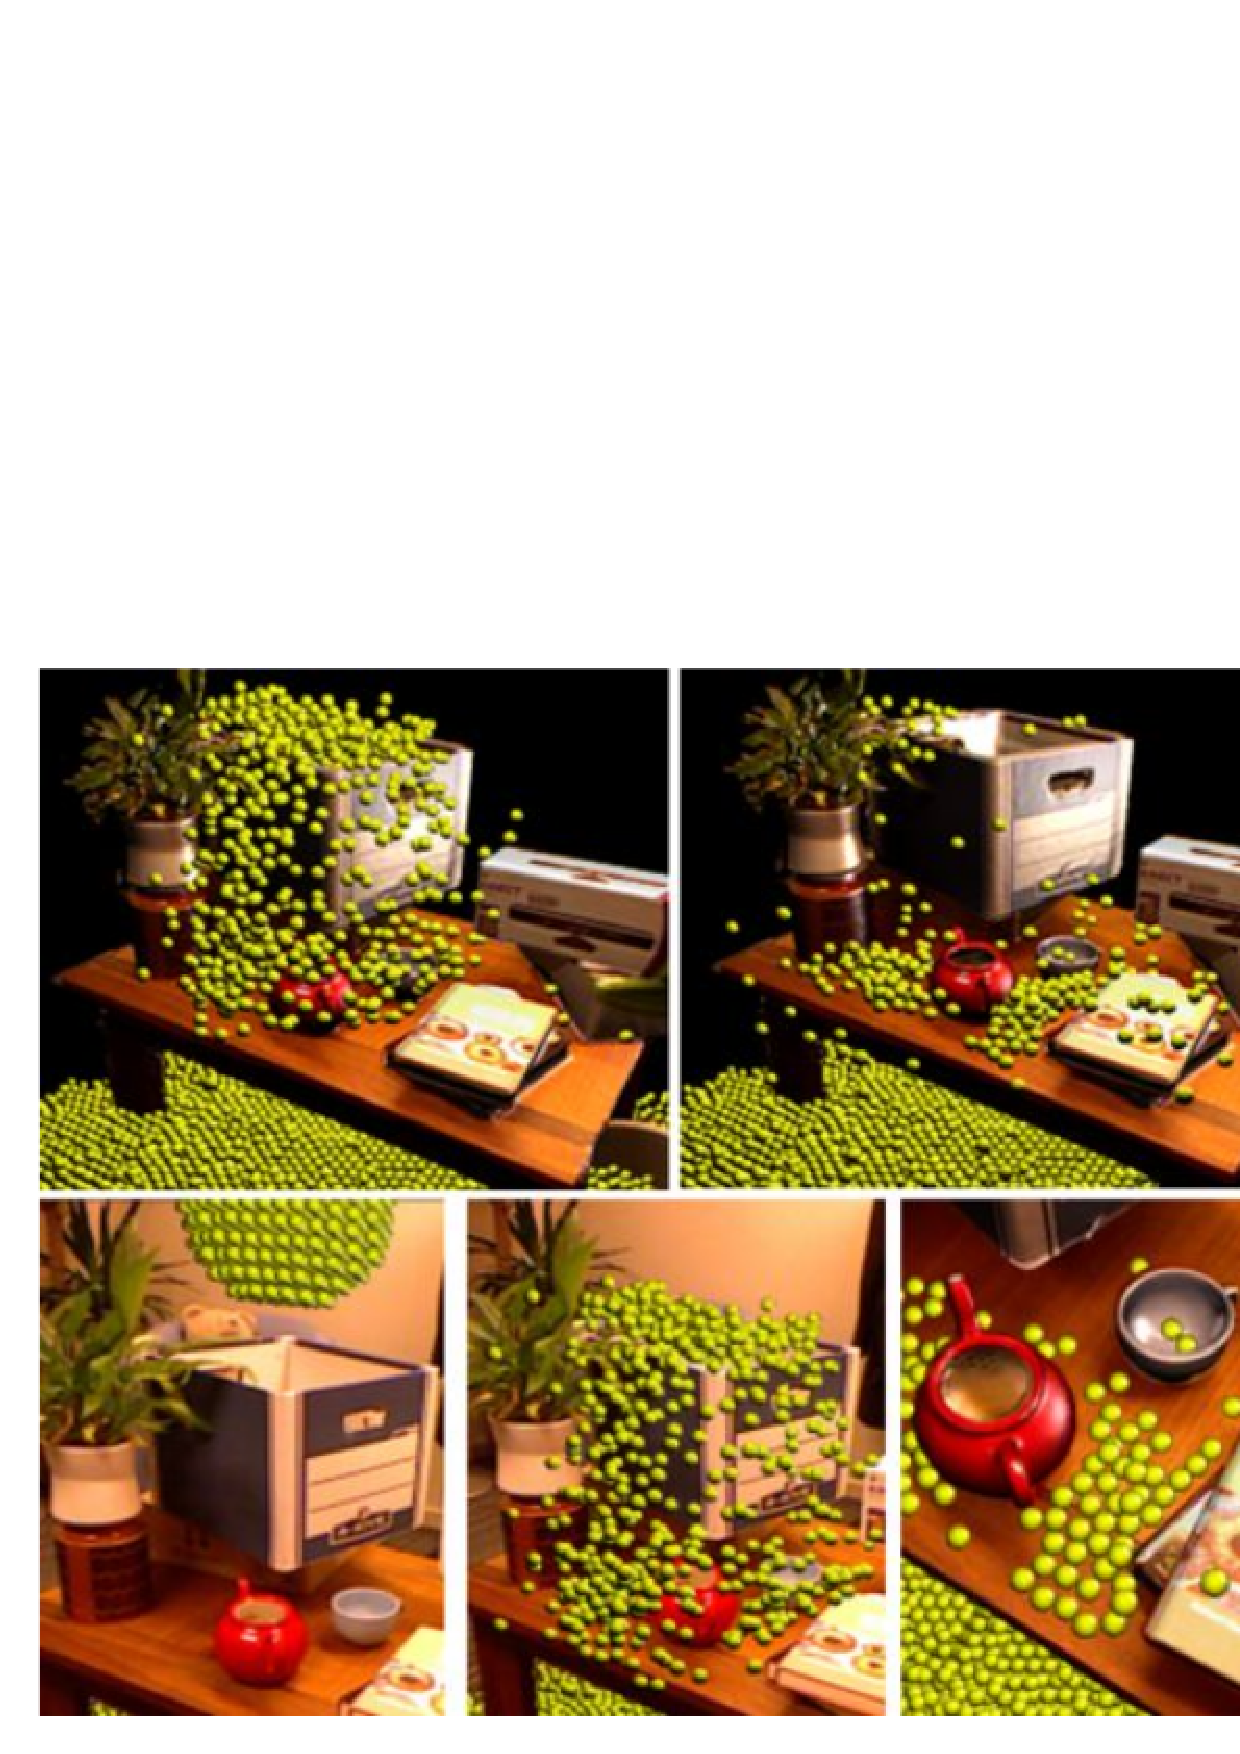
\includegraphics[scale=0.34]{images/izadi}
\caption{Reconstructed 3D scene with thousands of virtual particles}
\label{fig:izadi}
\end{center}
\end{figure}


All the 3D reconstruction methods can have problems with non lambertian 
surfaces and they need to make some assumptions about the surfaces reflectance. For example if we are using 
an infrared structured light pattern depth camera and the object that we are registering absorbs the infrared light, 
the reconstruction will fail. Similar problems can occur with laser scanners. 
Some materials such as glass or water can ruin the reconstruction.


%must be correctly located
In \cite{weise08} the user move the object using his hands in front of an RGB-D sensor (In-hand modeling), the hands are 
eliminated using a color skin detector and the user can see the reconstruction in real time, in order to correctly 
move the object.  The object is registered with Fast ICP, which instead of searching for the closest 
point, projects a transformated source point on the 2D target depth image in order to perform the matching. They use point
 to plane distance. This ICP variation is also used in \cite{jaeggli03}. \cite{weise08} uses geometrical and visual 
information to perform a correct registration. Imposing geometrical contraints based on the cameras lines of sight and visual 
contraints applying Gaussian derivative kernels to both images and measuring similarities.





